\documentclass[11pt,a4paper]{article}

\usepackage[margin=2.2cm]{geometry}
\usepackage[T1]{fontenc}
\usepackage[utf8]{inputenc}
\usepackage[french]{babel}
\usepackage{amsmath, amssymb}
\usepackage{booktabs}
\usepackage{graphicx}
\usepackage{hyperref}
\usepackage{float}
\usepackage{xcolor}
\usepackage{listings}

\hypersetup{colorlinks=true, linkcolor=blue, urlcolor=blue, citecolor=blue}

\lstdefinestyle{pythonstyle}{
  language=Python,
  basicstyle=\ttfamily\small,
  keywordstyle=\color{blue},
  commentstyle=\color{gray},
  stringstyle=\color{teal},
  showstringspaces=false,
  frame=single,
  breaklines=true,
  columns=fullflexible
}

\title{Programmation parallèle pour le Machine Learning :\\Parallélisation des arbres de décision et des random forests}
\author{Florian LAVA \and Léo-Paul MAROTTE\\3ème année ENSAE Paris}
\date{24 mai 2026}

\begin{document}

\maketitle

\begin{abstract}
Ce projet étudie la parallélisation des random forests en Python avec NumPy et joblib. Nous présentons le fonctionnement formel d'un arbre de décision, puis une implémentation séquentielle et parallèle d'une forêt aléatoire. Les expériences comparent 1, 2, 4 et 8 workers et montrent un speedup réel, mais sous-linéaire, en raison du coût de coordination et des limites imposées par la loi d'Amdahl.
\end{abstract}

\section{Introduction}

Ce projet s'inscrit dans la partie du cours consacrée à la programmation parallèle sur CPU. Sur un processeur multicœur, plusieurs tâches peuvent être exécutées simultanément si elles n'ont pas besoin de communiquer en permanence. Les random forests offrent précisément ce type de structure : les arbres sont appris indépendamment, à partir d'échantillons bootstrap différents.

L'objectif est double : proposer une implémentation pédagogique en Python et mesurer, de manière reproductible, les gains de performance obtenus par parallélisation. Le point important n'est pas seulement d'aller plus vite, mais de comprendre pourquoi le parallélisme fonctionne ici, ce qui reste séquentiel, et pourquoi le speedup n'est jamais parfaitement linéaire.

\subsection{Architecture et parallélisme}

Un CPU moderne contient plusieurs cœurs, chacun capable d'exécuter une suite d'instructions. Lorsqu'un programme se décompose en tâches indépendantes, celles-ci peuvent être réparties sur plusieurs workers. Dans notre cas, chaque worker entraîne un arbre complet. Il n'y a donc pas de race condition entre arbres pendant l'apprentissage, car chaque tâche travaille sur son propre sous-échantillon.

Le coût du parallélisme vient cependant de plusieurs sources : création des processus, copie ou sérialisation des données, ordonnancement des tâches et agrégation finale. Le gain observé dépend donc du rapport entre le travail utile par arbre et ce surcoût.

\section{Description mathématique}

\subsection{Arbre de décision}

Soit un ensemble d'apprentissage $S = \{(x_i, y_i)\}_{i=1}^n$ avec $y_i \in \{0,1\}$. Un arbre de décision cherche récursivement une variable $j$ et un seuil $t$ qui séparent les données en deux sous-ensembles :

\[
S_L = \{(x_i, y_i) : x_{ij} \le t\}, \qquad S_R = \{(x_i, y_i) : x_{ij} > t\}.
\]

Le critère retenu est l'impureté de Gini, qui mesure l'hétérogénéité d'un nœud. Si un nœud contient proportion $p$ de classe 1 et $1-p$ de classe 0, alors :

\[
G(S) = 1 - \sum_{k=0}^{1} p_k^2,
\]

où $p_k$ désigne la proportion de la classe $k$ dans $S$. Dans le cas binaire, si $p$ est la proportion de la classe 1, alors

\[
G(S) = 2p(1-p).
\]

Pour un split $(j,t)$, on minimise l'impureté pondérée :

\[
\Phi(j,t) = \frac{|S_L|}{|S|}G(S_L) + \frac{|S_R|}{|S|}G(S_R).
\]

Le meilleur split est celui qui minimise $\Phi(j,t)$ parmi les variables candidates et les seuils admissibles. Intuitivement, on cherche le seuil qui produit deux sous-groupes aussi purs que possible.

\subsection{Random forest}

Une random forest est un ensemble de $B$ arbres $h_1,\dots,h_B$. Chaque arbre est entraîné sur un bootstrap distinct et, à chaque nœud, sur un sous-ensemble aléatoire de variables. Le bootstrap introduit de la diversité entre arbres, ce qui réduit la corrélation de leurs erreurs. La prédiction finale est obtenue par vote majoritaire :

\[
\hat{y}(x) = \operatorname{mode}\bigl(h_1(x), \dots, h_B(x)\bigr).
\]

Le bootstrap et le sous-échantillonnage des variables réduisent la corrélation entre arbres et améliorent la robustesse de l'ensemble.

\subsection{Pourquoi la forêt est parallélisable}

L'entraînement de chaque arbre dépend uniquement des données d'entrée et d'une graine aléatoire. Les arbres peuvent donc être construits simultanément. Si $T_1$ est le temps séquentiel et si la part parallélisable représente une fraction $f$, la loi d'Amdahl donne :

\[
S(p) = \frac{1}{(1-f) + \frac{f}{p}},
\]

où $p$ est le nombre de workers. Cette formule montre qu'un speedup linéaire est impossible dès qu'une partie séquentielle subsiste. En pratique, le parallélisme ajoute aussi un surcoût de sérialisation, de création de processus et d'ordonnancement.

Dans cette implémentation, joblib utilise le backend \texttt{loky}, qui s'appuie sur des processus séparés. Ce choix est adapté aux calculs CPU intensifs, car il évite les limites du GIL de Python pour l'exécution parallèle de code pur Python.

\section{Implémentation}

Le projet repose sur trois briques : génération d'un jeu de données artificiel, implémentation d'un arbre de décision séquentiel, puis entraînement parallèle de la forêt via joblib.

Le jeu de données synthétique est volontairement non linéaire : certaines variables sont informatives, d'autres sont du bruit, et la frontière de décision dépend d'interactions non triviales. Cela rend le benchmark plus réaliste qu'un problème artificiellement simple.

Le premier extrait montre comment l'algorithme choisit un split :

\begin{lstlisting}[style=pythonstyle]
for feature_index in candidate_features:
  feature_impurity, threshold = self._best_split_for_feature(
    X[:, feature_index],
    y_binary,
  )
  if threshold is not None and feature_impurity < best_impurity:
    best_impurity = feature_impurity
    best_feature = int(feature_index)
    best_threshold = threshold
\end{lstlisting}

Cette boucle parcourt un sous-ensemble de variables candidates et compare les seuils possibles via le critère de Gini. Le coût principal est le tri de la variable et l'évaluation des coupures admissibles.

Le deuxième extrait illustre le découpage du travail entre workers :

\begin{lstlisting}[style=pythonstyle]
if self.n_jobs == 1:
    trees = [self._fit_one_tree(X, y, int(seed)) for seed in seeds]
else:
    trees = Parallel(n_jobs=self.n_jobs, backend="loky")(
        delayed(self._fit_one_tree)(X, y, int(seed)) for seed in seeds
    )
\end{lstlisting}

Chaque tâche correspond à l'entraînement complet d'un arbre sur un bootstrap. L'agrégation finale ne nécessite qu'un vote majoritaire, sans communication fine entre workers, ce qui limite les verrous et les synchronisations.

La génération de données est volontairement non linéaire afin d'obtenir un problème réaliste : variables informatives, bruit additif et frontière de décision non triviale.

\section{Résultats expérimentaux}

Les mesures sont effectuées pour 1, 2, 4 et 8 workers sur un problème synthétique de classification binaire. Avant chaque série de mesures, un petit entraînement d'échauffement est effectué afin de réduire l'effet du démarrage des processus et de stabiliser les temps observés. Chaque configuration est ensuite répétée plusieurs fois, puis on calcule la moyenne et l'écart-type des temps d'entraînement.

Le tableau ci-dessous est généré à partir des résultats du benchmark, afin d'éviter toute incohérence entre le texte, le CSV et les figures.

\begin{table}[H]
\centering
\begin{tabular}{rrrrr}
\toprule
Workers & Temps moyen (s) & Écart-type (s) & Accuracy moyenne & Speedup \\
\midrule
1 & 4.790 & 0.015 & 0.850 & 1.00 \\
2 & 2.614 & 0.036 & 0.850 & 1.83 \\
4 & 1.989 & 0.039 & 0.850 & 2.41 \\
8 & 1.732 & 0.063 & 0.850 & 2.77 \\

\bottomrule
\end{tabular}
\caption{Résultats du benchmark séquentiel/parallèle.}
\end{table}

Sur ce jeu de données, le speedup continue d'augmenter jusqu'à 8 workers, mais de façon sous-linéaire. Autrement dit, ajouter des workers améliore encore le temps total, mais chaque worker supplémentaire apporte un gain marginal plus faible.

On observe aussi que l'accuracy reste stable d'une configuration à l'autre. C'est un point important : le parallélisme accélère l'entraînement, mais ne modifie pas la règle de décision apprise par l'algorithme.

Le speedup vaut $S(p)=T(1)/T(p)$. Une efficacité utile est $E(p)=S(p)/p$, égale à $1$ dans le cas idéal. Ici, $E(8)$ reste inférieur à $E(4)$, ce qui montre que le gain obtenu en ajoutant des workers devient de moins en moins efficace.

Du point de vue de la mesure, il faut interpréter ces résultats comme des ordres de grandeur plutôt que comme des constantes absolues : l'ordonnancement du système, l'état de la machine et la variabilité du multiprocessing influencent les temps observés. C'est précisément pour cette raison qu'un protocole avec plusieurs répétitions est préférable à une mesure unique.

Les figures suivantes illustrent la variation du temps d'entraînement et du speedup en fonction du nombre de workers.

\begin{figure}[H]
\centering
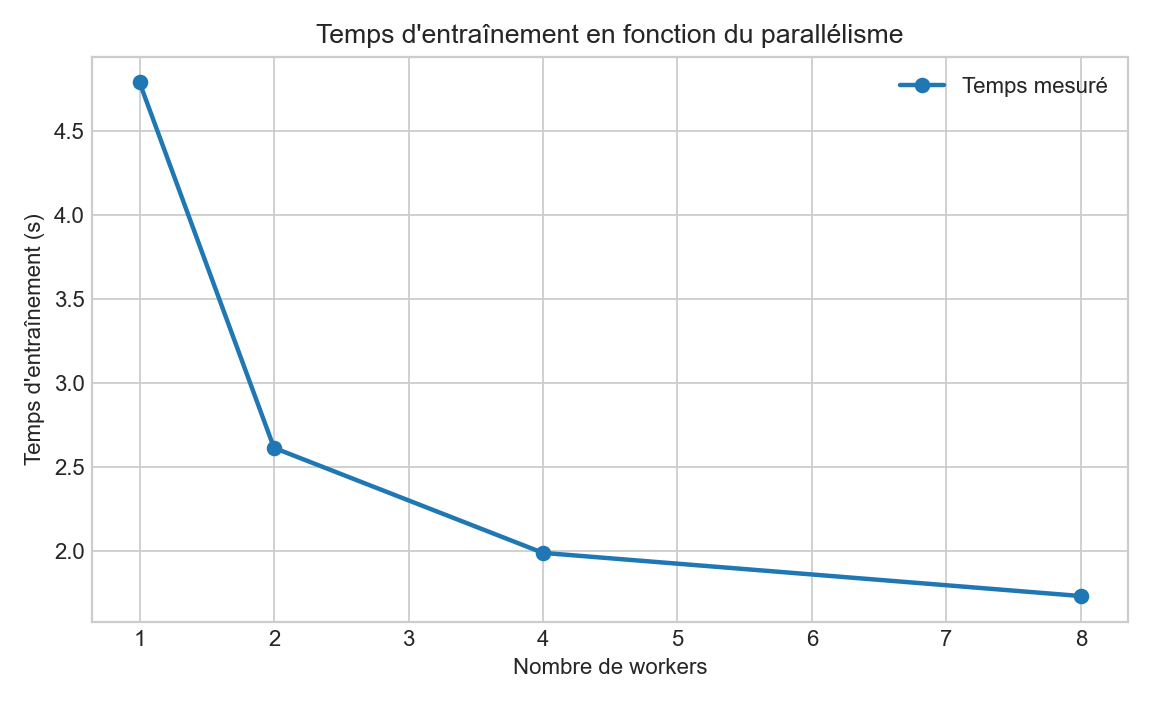
\includegraphics[width=0.82\linewidth]{figures/time_vs_workers.png}
\caption{Temps d'entraînement en fonction du nombre de workers.}
\end{figure}

\begin{figure}[H]
\centering
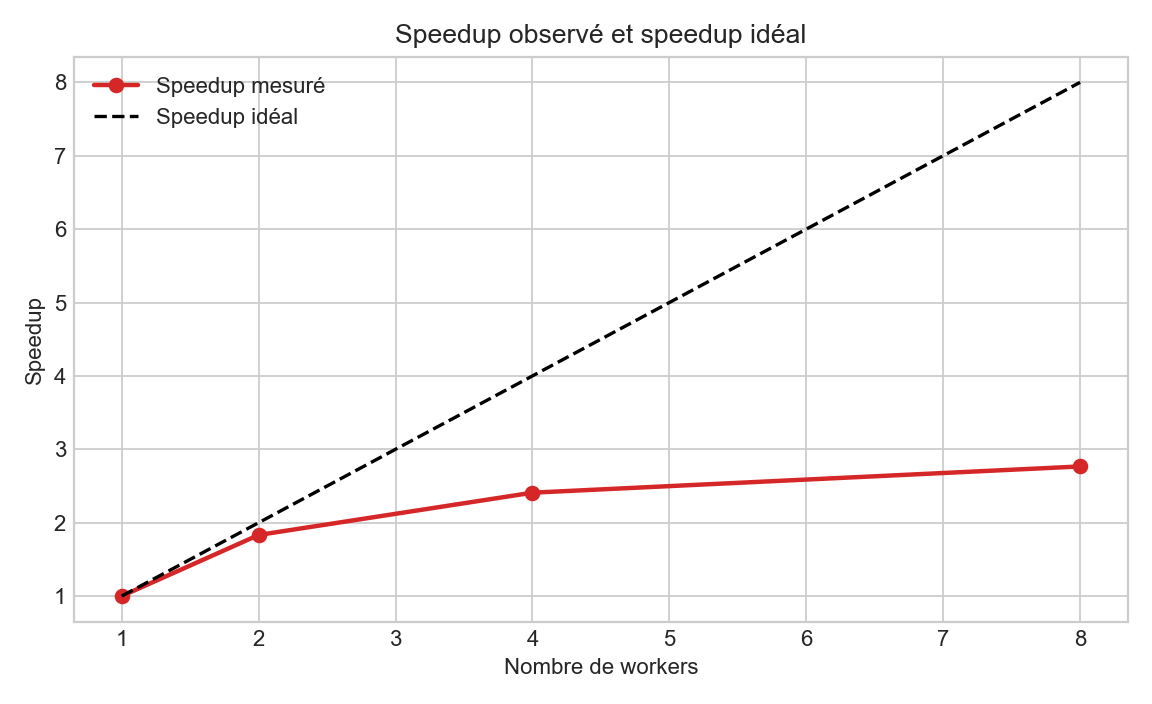
\includegraphics[width=0.82\linewidth]{figures/speedup_vs_workers.png}
\caption{Speedup observé et speedup idéal.}
\end{figure}

La tendance observée est conforme à l'analyse théorique : le temps diminue lorsque le nombre de workers augmente, mais le speedup reste sous-linéaire. Les principales causes sont les suivantes :

\begin{itemize}
  \item le temps séquentiel incompressible du code Python et de la construction de certains objets,
  \item le coût du multiprocessing et de la sérialisation des tableaux NumPy,
  \item le déséquilibre possible entre arbres si certains splits sont plus coûteux que d'autres,
  \item la mémoire supplémentaire consommée par la duplication des données dans les processus.
\end{itemize}

\section{Conclusion}

Les random forests sont naturellement parallélisables car les arbres sont indépendants au moment de l'entraînement. L'implémentation proposée avec joblib montre un gain réel, et le benchmark confirme une accélération jusqu'à 8 workers, mais le speedup demeure inférieur à la courbe idéale en raison de la partie séquentielle, des coûts de communication et de l'ordonnancement des processus.

Le projet met ainsi en évidence le point essentiel du cours : la parallélisation est particulièrement efficace lorsque les tâches sont indépendantes, mais son efficacité reste contrainte par l'architecture mémoire et par le coût du parallélisme lui-même.

Les perspectives naturelles seraient d'étudier des jeux de données plus grands, de comparer différents backends de joblib, ou d'explorer une version GPU pour montrer où se situent les gains de parallélisme quand la structure de calcul change.

\end{document}
